\section{Mollification of sets of least perimeter}\label{MollifierSection}
In this section our goal is to show that given a set $U$ of least perimeter in $\Hyp^d$, we can find a $C^1$ hypersurface $N$ which approximates $\partial^* U$ arbitrarily well in the following sense:

\begin{proposition}\label{mollifier quant}
    For every $\varepsilon > 0$ there exists $\gamma^* > 0$ with the following property:

    For every $P \in \Hyp^d$, every $\delta > 0$, and every set $U$ of least perimeter in $B_\delta$, such that
    \begin{equation}\label{bootstrap the mollifier}
    \gamma := \delta^{1 - d}\int_{B_\delta} *(|\dif 1_U| - x\partial_z 1_U) < \gamma^*,
    \end{equation}
    where $B_r = B(P, r)$, and almost every $t \in (0, \delta)$, there exists a set $V$ of $C^1$ perimeter in $B_t$, such that
    \begin{align}
    |V \cap B_t| &\leq \eta(V, B(P, t)) + \varepsilon \delta^{d - 1} \gamma, \label{mollifier quant1}\\
    \left||U \cap B_t| - |V \cap B_t|\right| &\leq \varepsilon \delta^{d - 1} \gamma, \label{mollifier quant2}\\
    (\normal_V, x\partial_z) &\geq (1 - \varepsilon) \text{ on } B_{t-\varepsilon}, \label{mollifier quant4}
    \end{align}
    and for every vector field $Y$ defined near $P$ with $|Y| \sim 1$ and $|\Div Y| \lesssim 1$,
    \begin{equation}
    \left|\int_{B_t} *Y(1_U - 1_V)\right| \leq \varepsilon \delta^{d - 1} \gamma. \label{mollifier quant3}
    \end{equation}
\end{proposition}

For the proof of Proposition \ref{mollifier quant} we follow \cite[Chapter 7]{Giusti77}; in particular we use Giusti's convolution kernel rather than the Gaussian kernel used by Miranda, given as follows:

\begin{definition}
For a function $u \in L^1_\loc$ defined near $O$ and $\varepsilon > 0$ small, we defined
$$u_\varepsilon(x) := \frac{d(d + 1)}{|\Sph^{d - 1}| \varepsilon^d} \int_0^\varepsilon r^{d - 1}(1 - r/\varepsilon) \int_{\Sph^{d - 1}} u(x - \Phi_r(\theta)) \dif \theta \dif r.$$
We denote by $\chi_\varepsilon$ the convolution kernel
$$\chi_\varepsilon = \frac{d(d + 1)}{|\Sph^{d - 1}| \varepsilon^d}r^{d - 1}(1 - r/\varepsilon) \dif \theta \dif r.$$
\end{definition}

Thus $\chi_\varepsilon$ is a probability measure on $(0, \varepsilon) \times \Sph^{d - 1}$ which converges in the weakstar topology to the Dirac measure at the origin.
We record two technical lemmata which easily follow from \cite[Lemmata 7.1--7.2]{Giusti77} by multiplying the volume form by a constant:

\begin{lemma}\label{Giusti71}
Suppose that $u = 1_U$ is a Borel indicator function defined near $O$. Then $u_\varepsilon \in C^1$, and there exists an absolute constant $c > 0$ such that for every $\rho > 0$ small and $x \in \Hyp^d$, if
$$c\rho^2 < u_\varepsilon(x) < 1 - c\rho^2,$$
then
\begin{equation}\label{Giusti71 claim}
d(x, \partial^* U) < \varepsilon(1 - \rho).
\end{equation}
\end{lemma}

\begin{lemma}\label{Giusti72}
Let $u \in BV(\{r < \delta\})$ and $\tau, \varepsilon > 0$. If $\tau + \varepsilon < \delta$, then
\begin{align*}
\int_{\{r < \tau\}} *|u_\varepsilon - u| &\lesssim \varepsilon \int_{\{r < \tau + \varepsilon\}} *|\dif u|\\
\int_{\{r < \tau\}} *(|\dif u_\varepsilon| - |\dif u|) &\lesssim \int_{\{\tau < r < \tau + \varepsilon\}} *|\dif u|.
\end{align*}
\end{lemma}

The main step in the proof of Proposition \ref{mollifier quant} is to generalize \cite[Theorem 7.3, Remark 7.4]{Giusti77}.

\begin{lemma}\label{main mollifier lemma}
Let $\gamma, p > 0$, let $U$ be a set of least perimeter, $u = 1_U$, and suppose that
\begin{equation}\label{hypothesis on main mollifier lemma}
\int_{B_1} *(|\dif u| - x\partial_z u) \leq \gamma.
\end{equation}
Let $\varepsilon = \gamma^p$, $\sigma = \gamma^{1/(2(d - 1))}$, and $\varphi = u_\varepsilon$. Then there exists $c > 0$ and $q > 0$ independent of $\gamma$ or $u$, but allowed to depend on $p$, such that on the set $\{r < \sigma\} \cap \{c\gamma^2 < \varphi < 1 - c\gamma^2\}$,
\begin{equation}\label{claim on main mollifier lemma}
|\dif \varphi| - x\partial_z \varphi \lesssim_p \gamma^q |\dif \varphi|,
\end{equation}
and for every $y \in (c\gamma^2, 1 - c\gamma^2)$ the level set $\partial \{\varphi > y\} \cap \{r < \sigma\}$ is a $C^1$ hypersurface.
\end{lemma}

The proof of this result is quite long and so we break it up into sublemmata.
To set them up, let $\delta = \gamma^d > 0$ and select disjoint balls $V_1/2, \dots, V_N/2$, centered on $Q_n$, in $\partial^* U \cap B_{\varepsilon(1 - 2\delta)}$ of radius $\delta\varepsilon$ so that the dilates $V_n$ cover $\partial^* U \cap B_{\varepsilon(1 - 2\delta)}$.
It is easy to show that such a cover exists, because $\overline{\partial^* U \cap B_{\varepsilon(1 - 2\delta)}}$ is compact if $\gamma$ is small enough, so for such a $\gamma$ we can greedily select $Q_n \in \overline{\partial^* U \cap B_{\varepsilon(1 - 2\delta)}}$ to maximize $\min(d(Q_1, Q_n), \dots, d(Q_{n - 1}, Q_n))$.
We set $V_0 = B_\varepsilon \setminus B_{\varepsilon(1 - 2\delta)}$.
Since $\dif u$ is supported in $\bigcup_n V_n$,
$$|\dif \varphi|(x) - x\partial_z \varphi(x) = (|\dif u| - x\partial_zu)_\varepsilon \leq \sum_{n=0}^N \int_{V_n} (1_{V_n}(|\dif u| - x\partial_zu))_\varepsilon.$$
We estimate each of the terms in this sum in turn:

\begin{figure}[ht]
\caption{The sets $V_0, V_1/2 \dots, V_n/2$ (in dark grey) are an annulus and several small balls of radius $\delta$, which approximately cover the boundary of the set $U$ (in light grey).}
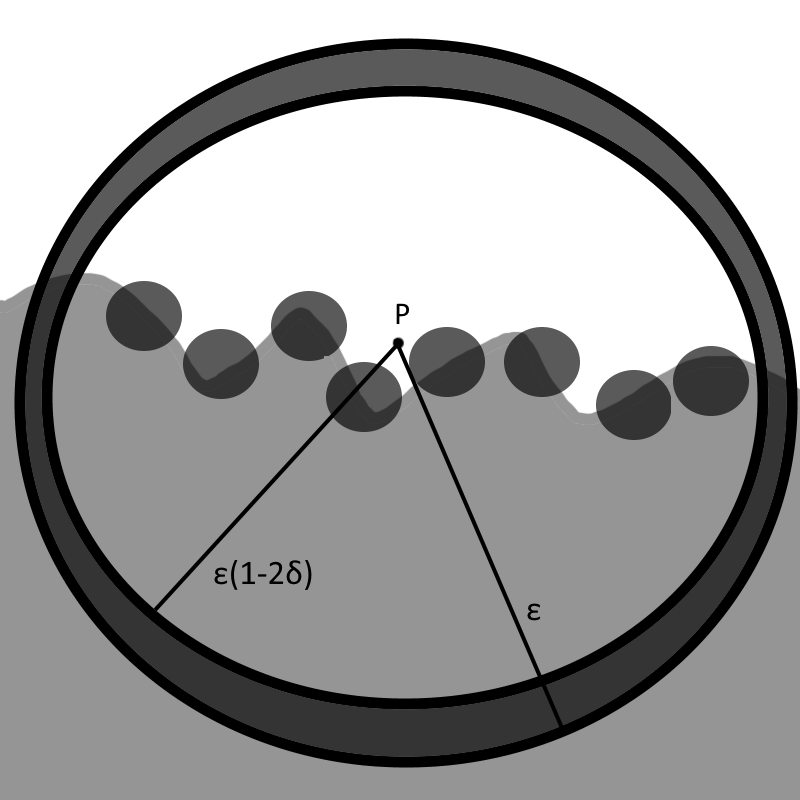
\includegraphics[width=0.4\textwidth]{covering lemma}
\end{figure}


If we write $F$ for the Radon-Nikod\'ym derivative of $\chi_\varepsilon$ with respect to the usual measure on $\Hyp^d$, then for every $x, z$ close to $O$ and $y \in B(z, \delta)$,
\begin{equation}\label{approximation of mollifier 2}
F(x - y) \sim \frac{1}{\varepsilon^d}\left(1 - \frac{d(x, Q)}{\varepsilon}\right)
\end{equation}
uniformly as $\delta, \varepsilon \to 0$. TODO: Clean me up

\begin{sublemma}
For every $n \geq 1$, if $r < \sigma$ then
$$\int_{V_n} \chi_\varepsilon(x - \cdot)(|du| - Xu) \lesssim_{g, p, P} \gamma^{O(1)} \int_{V_n/2} \chi_\varepsilon(x - \cdot)|du|.$$
\end{sublemma}
\begin{proof}
By (\ref{approximation of mollifier 2}), if $\gamma$ is small enough depending on $g$\footnote{One might worry that we frequently rescale $g$ in this paper.
However, in all of our rescalings, the curvature tensor remains in some bounded set, so these rescalings will never send $\gamma$ to $0$.}, then for every $y \in 2V_n$,
\begin{align*}
\int_{2V_n} \chi_\varepsilon(x - \cdot)(|du| - Xu) &\lesssim F_n(x) \int_{2V_n} |du| - Xu ~\vol, \\
F_n(x) &:= \frac{1}{\varepsilon^d}\left(1 - \frac{d(x, Q_n)}{\varepsilon}\right).
\end{align*}
If $\gamma$ is chosen small enough, then $\sigma > 2\delta\varepsilon$ and so if we set $W_n = B(Q_n, \sigma)$ and apply Proposition \ref{Monotonicity Formula},
\begin{align*}
\int_{2V_n}|du| - Xu ~\vol &\leq
B \left[\sigma^{1 - d}\int_{W_n} |du| - Xu ~\vol + \sigma^{1 - d}\int_{W_n} Xu ~\vol - (2\delta\varepsilon)^{1 - d}\int_{2V_n} Xu ~\vol \right],\\
B &:= e^{O(1)(\sigma^2 - 4\delta^2\varepsilon^2)}(2\delta\varepsilon)^{d - 1}.
\end{align*}
From Taylor's theorem and the fact that $\sigma > 2\delta\varepsilon$,
\begin{align*}
B \lesssim \delta^{d - 1} \varepsilon^{d - 1} + \sigma^2 \delta^{d - 1} \varepsilon^{d - 1} \lesssim \delta^{d - 1} \varepsilon^{d - 1}
\end{align*}
if $\gamma$ is small.
By (\ref{hypothesis on main mollifier lemma}),
$$\sigma^{1 - d}\int_{W_n} |du| - Xu ~\vol \leq \gamma^{\frac{1 - d}{2(d - 1)} + 1} = \gamma^{1/2}.$$
By Proposition \ref{Monotonicity Formula},
\begin{align*}
\sigma^{1 - d}\int_{W_n} Xu ~\vol - (2\delta\varepsilon)^{1 - d}\int_{2V_n} Xu ~\vol &\lesssim \sigma + (1 + \alpha)\sqrt{\sigma^{1 - d} \int_{W_n} |du| ~\vol - (2\delta\varepsilon)^{1 - d} \int_{2V_n} |du| ~\vol},\\
&\alpha := (d - 1)\log \frac{\sigma}{2\delta\varepsilon}.
\end{align*}

By Corollary \ref{scalar curvature monotonicity},
$$\sigma^{1 - d} \int_{W_n} X u ~\vol - (2\delta\varepsilon)^{1 - d} \int_{2V_n} |du| ~\vol \lesssim \sigma^2,$$
so by (\ref{hypothesis on main mollifier lemma}),
\begin{align*}
\sigma^{1 - d} \int_{W_n} |du| ~\vol - (2\delta\varepsilon)^{1 - d} \int_{2V_n} |du| ~\vol &= \sigma^{1 - d} \int_{W_n} |du| - Xu ~\vol \\
&\qquad + \sigma^{1 - d} \int_{W_n} Xu ~\vol - (2\delta\varepsilon)^{d - 1} \int_{W_n} |du| ~\vol \\
&\leq \gamma + O(\sigma^2) \lesssim \sigma^2.
\end{align*}
It follows from the definitions that
$$(1 + \alpha)\sigma \lesssim -\gamma^{1/2(d - 1)} \log \gamma \lesssim \gamma^{1/3(d - 1)}.$$
Summing up everything in this step of the proof thus far,
\begin{equation}\label{big bound 1}
\int_{2V_n} \chi_\varepsilon(x - \cdot)(|du| - Xu) ~\vol \lesssim \delta^{d - 1} \varepsilon^{d - 1} F_n(x) \gamma^{1/3(d - 1)}.
\end{equation}
Since $U$ has least perimeter, Proposition \ref{doubling dimension} implies that
$$\delta^{d - 1} \varepsilon^{d - 1} \lesssim \int_{V_n} |du| ~\vol,$$
so by (\ref{approximation of mollifier 2}, \ref{big bound 1}),
\begin{align*}
\int_{2V_n} \chi_\varepsilon(x - \cdot)(|du| - Xu) ~\vol
&\lesssim \gamma^{1/3(d - 1)} \int_{V_n} \chi_\varepsilon(x - \cdot)|du|.
\qedhere \end{align*}
\end{proof}

\begin{sublemma}
One has
$$\int_{V_0} \chi_\varepsilon(x - \cdot)(|du| - Xu) \lesssim_{g, p, P} \gamma^{O(1)} \int_{B_\varepsilon} \chi_\varepsilon(x - \cdot)|du|$$
provided that $x = (r, \Theta)$ satisfies $r < \sigma$ and $\varphi \in (o(\gamma), 1 - o(\gamma))$.
\end{sublemma}
\begin{proof}
From (\ref{approximation of mollifier 2}) it easily follows that for $y \in V_0$, $\chi_\varepsilon(x - y)/\vol(x - y) \lesssim \frac{\delta}{\varepsilon^d}$,
whence, by minimality of $\partial^* U$,
\begin{align*}
\int_{V_0} \chi_\varepsilon(x - \cdot)(|du| - Xu) &\lesssim \frac{\delta}{\varepsilon^d} \int_{B_\varepsilon} |du| ~\vol \lesssim \frac{\delta}{\varepsilon^d} |\partial B_\varepsilon| \lesssim \frac{\delta}{\varepsilon}.
\end{align*}
By Lemma \ref{Giusti71}, there exists $c > 0$ such that if $\varphi \in (c\gamma^2, 1 - c\gamma^2)$, then $d(x, \partial U) < \varepsilon(1 - \gamma)$, so in particular we can find $Q \in \partial^* U$ such that $d(x, Q) < \varepsilon(1 - \gamma)$.
If $d(y, Q) < \gamma\varepsilon/2$, then
$$d(x, y) \leq \varepsilon - \gamma\varepsilon + \frac{\gamma\varepsilon}{2} \leq \varepsilon - \frac{\gamma\varepsilon}{2},$$
so by (\ref{approximation of mollifier 2}), $\chi_\varepsilon(x - y)/\vol(x - y) \gtrsim \frac{\gamma}{\varepsilon^d}$
for every $y \in B(Q, \gamma\varepsilon/2)$.
In particular, since $\delta = \gamma^d$, minimality of $\partial^* U$ gives
\begin{align*}
\int_{V_0} \chi_\varepsilon(x - \cdot)(|du| - Xu) &\lesssim \frac{\delta}{\gamma^{d - 1}} \frac{\gamma^{d - 1}}{\varepsilon}\\
&\lesssim \gamma |\partial B(Q, \gamma\varepsilon/2)| \int_{B(Q, \gamma\varepsilon/2)} \chi_\varepsilon(x - \cdot) \\
&\lesssim \gamma \int_{B(Q, \gamma\varepsilon/2)} \chi_\varepsilon(x - \cdot) |du|\\
&\lesssim \gamma \int_{B_\varepsilon} \chi_\varepsilon(x - \cdot) |du|. \qedhere
\end{align*}
\end{proof}

\begin{proof}[Proof of Lemma \ref{main mollifier lemma}]
Since the balls $V_n$ are disjoint, we can sum over $n$ to obtain
\begin{equation}\label{claim on main mollifier lemma 2}|d\varphi|(x) - X\varphi(x) \lesssim_{g, p, P} \gamma^{O(1)} \int_{B_\varepsilon} \chi_\varepsilon(x - \cdot)|du| \leq \gamma^{O(1)} |d\varphi|(x),
\end{equation}
which implies (\ref{claim on main mollifier lemma}). Thus we may fix
$$x \in \partial^* U \cap \{r < \sigma\} \cap \{\varphi \in (f(\gamma), 1 - f(\gamma)),$$
and choose $\gamma$ so small that (\ref{claim on main mollifier lemma 2}) simplifies to $X\varphi(x) \gtrsim |d\varphi(x)|$.
Thus, in particular,
$$X\varphi(x) \gtrsim \int_{B_\varepsilon} \chi_\varepsilon(x - \cdot) |du| > 0.$$
By Lemma \ref{Giusti71}, $d\varphi$ is continuous, so the level sets of $\varphi$ must be $C^1$.
\end{proof}

We now set up the proof of Proposition \ref{mollifier quant}.
After rescaling, we may fix a sequence $(u_n)$ of indicator functions of sets $(U_n)$ with least perimeter in $B_1$.
We define
$$\gamma_n := \int_{B_1} |\dif u_n| - x\partial_z u_n,$$
assume that $(\gamma_n) \in \ell^1$, and draw $t \in (0, 1)$ uniformly at random.
It now suffices to show that
\begin{align}
|\partial V_n \cap B_t| &\leq \eta(V_n, B_t) + o(\gamma_n), \label{mollifier prop1}\\
\left|\int_{B_t} |\dif u_n| - |\dif v_n| ~\vol\right| &\ll \gamma_n, \label{mollifier prop2}\\
\lim_{n \to \infty} g(\normal_{V_n}, X) &= 1, \label{mollifier prop4}
\end{align}
where the limit in (\ref{mollifier prop4}) is uniform, and for every vector field $Y$ with $|Y| \sim 1$ and $|\Div Y| \lesssim 1$,
\begin{equation}
\left|\int_{B_t} Y(u_n - v_n)~\vol\right| \lesssim \gamma_n^2. \label{mollifier prop3}
\end{equation}

Let $w_n = (u_n)_{\gamma_n^4}$, let $c$ be the constant given by Lemma \ref{main mollifier lemma}, and let $a_n = c\gamma_n$, $b_n = 1 - c\gamma_n$.
0By Proposition \ref{Coarea2},
$$\int_{B_t} |dw_n| ~\vol = \int_0^1 |\partial^* \{w_n > y\} \cap B_t| ~dy \geq \int_{a_n}^{b_n} |\partial^* \{w_n > y\} \cap B_t| ~dy.$$
By the mean value theorem, there exists $y_n \in (a_n, b_n)$ such that
\begin{equation}\label{MVT mollifier}
|\partial^* \{w_n > y_n\} \cap B_t| \leq \frac{1}{b_n - a_n} \int_{B_t} |dw_n| ~\vol.
\end{equation}
If set $V_n = \{w_n > y_n\}$, $v_n = 1_{V_n}$, then $V_n$ has $C^1$ boundary in $B_t$ by definition of $a_n, b_n$, and from (\ref{claim on main mollifier lemma}), the locally uniform convergence (\ref{mollifier prop4}) holds.

So it remains to show that (\ref{mollifier prop1}--\ref{mollifier prop3}) hold almost surely.
Towards this end we will later show that
\begin{align}
|\partial V_n \cap B_t| &\leq |\partial^* U_n \cap B_t| + o(\gamma_n), \label{approximation of surface area} \\
\int_{\partial B_t} |u_n - v_n| ~\vol_{\partial B_t} &\lesssim \gamma_n^2. \label{approximation of volume}
\end{align}
If (\ref{approximation of surface area}, \ref{approximation of volume}) are true,
then by (\ref{a priori estimate 3}, \ref{approximation of volume}),
$$|\partial^* U_n \cap B_t| \leq |\partial V_n \cap B_t| + o(\gamma_n)$$
so by (\ref{approximation of surface area}), (\ref{mollifier prop2}) holds.
From an integration by parts using the estimate $1/2 \leq g(Y, Y) \leq 2$, and (\ref{approximation of volume}),
\begin{align*}
\left|\int_\Omega Y(u_j - v_j) ~\vol\right|
&\leq \left|\int_{\partial \Omega} (u_j - v_j)g(Y, \normal) ~\vol_{\partial \Omega}\right| \\
&\lesssim \int_{\partial \Omega} |u_j - v_j| ~\vol_{\partial \Omega} \lesssim \gamma_n^2
\end{align*}
which gives (\ref{mollifier prop3}).
By the fact that $U_n$ has least perimeter, and (\ref{a priori estimate 1}, \ref{mollifier prop2}),
\begin{align*}
|\partial V_n \cap B_t| &\leq |\partial U_n \cap B_t| + o(\gamma_n) \\
&= \eta(U_n, B_t) + o(\gamma_n)\\
&\leq \eta(V_n, B_t) + \int_{\partial B_t} |u_n - v_n| ~\vol_{\partial B_t} + o(\gamma_n),
\end{align*}
so by (\ref{approximation of volume}), (\ref{mollifier prop1}) holds.

%%%%%%%%%%%%%%%%%%%%%%%%%%%%%%%%%%%%%%%%%%%%%%%%%%%%%%%%%%%%%%%%

\begin{proof}[Proof of (\ref{approximation of surface area})]
By Lemma \ref{Giusti72}, one has
\begin{equation}\label{Giusti 720a}
\limsup_{n \to \infty} \int_{B_t} |du_n| - |dw_n| ~\vol \leq \limsup_{n \to \infty} \int_{B_{t + \gamma_n^4} \setminus B_t} |du_n| ~\vol.
\end{equation}
If we define $\mu = \sum_n \gamma_n|du_n| ~\vol$, then $\mu(B_1) < \infty$, since $(\gamma_n) \in \ell^1$ and $|\partial^* U_n \cap B_1|$ is uniformly bounded (c.f. Proposition \ref{doubling dimension}).
The hypotheses of \cite[(7.20)]{Giusti77} are (\ref{Giusti 720a}) and the fact that $\mu$ is a finite Borel measure on $B_1$, and the conclusion is that almost surely,
\begin{equation}\label{Giusti 720b}
\limsup_{n \to \infty} \gamma_n^{-2} \int_{B_t} |dw_n| - |du_n| ~\vol \leq 0.
\end{equation}
From (\ref{MVT mollifier}, \ref{Giusti 720b}), one has (\ref{approximation of surface area}).
\end{proof}

\begin{proof}[Proof of (\ref{approximation of volume})]
Let
$$f_n(t) = \gamma_n^{-4} \int_{B_t} |u_n - w_n| ~\vol.$$
By Lemma \ref{Giusti72} and the fact that $U_j$ has least perimeter in $B_1$,
$$\limsup_{n \to \infty} f_n(t) \leq \limsup_{n \to \infty} \int_{B_1} |du_n| ~\vol \leq |\partial B_1|.$$
Moreover, $f_n$ is monotone.
This implies that almost surely, $f_n'(t)$ is uniformly bounded in $n$.
But
$$f_n'(t) = \gamma_n^{-4} \int_{\partial B_t} |u_n - w_n| ~\vol_{\partial B_t},$$
so
\begin{equation}\label{mollify cubic gamma}
\int_{\partial B_t} |u_n - w_n| ~\vol_{\partial B_t} \lesssim \gamma_n^4.
\end{equation}
We now set $z_n = \min(y_n, 1 - y_n)$ and estimate
\begin{align*}
\int_{\partial B_t} |u_n - v_n| ~\vol_{\partial B_t} &= |\partial B_t \cap U_n \Delta V_n| \\
&= |\partial B_t \cap V_n \setminus U_n| + |\partial B_t \cap U_n \setminus V_n| \\
&\leq \frac{y_n}{z_n} |\partial B_t \cap V_n \setminus U_n| + \frac{1 - y_n}{z_n} |\partial B_t \cap U_n \setminus V_n|.
\end{align*}
From definition of $V_n$, $w_n - u_n > y_n$ on $V_n \setminus U_n$ and $u_n - w_n > 1 - y_n$ on $U_n \setminus V_n$, so
\begin{align*}
\int_{\partial B_t} |u_n - v_n| ~\vol_{\partial B_t} &\leq z_n^{-1} \int_{\partial B_t \cap U_n \setminus V_n} |u_n - w_n| ~\vol_{\partial B_t} + z_n^{-1}\int_{\partial B_t \cap V_n \setminus U_n} |u_n - w_n| ~\vol_{\partial B_t} \\
&\leq z_n^{-1} \int_{\partial B_t} |u_n - w_n| ~\vol_{\partial B_t}.
\end{align*}
But
$$z_n^{-1} \leq \max(y_n^{-1}, (1 - y_n)^{-1}) \leq \max(a_n^{-1}, b_n^{-1}) \lesssim \gamma_n^{-2}$$
whence
$$\int_{\partial B_t} |u_n - v_n| ~\vol_{\partial B_t} \lesssim \gamma_n^{-2} \int_{\partial B_t} |u_n - w_n| ~\vol_{\partial B_t},$$
so by (\ref{mollify cubic gamma}), (\ref{approximation of volume}) holds.
\end{proof}
